微分方程及相关学科几乎贯穿各类科学研究，是现代数学的重要分支，也是解决实际问题的工具。与代数方程不同：代数方程寻求\textbf{未知量与已知量}的关系；微分方程还涉及\textbf{未知量的变化率（导数）}，描述"变化问题"。例如，自由落体关心"下落距离如何随时间变化"；火箭关心"飞行轨道如何随时间演化"。

\textbf{基本思想}：找出已知函数与未知函数的关系，从含未知函数及其导数的方程中求得未知函数表达式。

\textbf{历史}：微分方程与微积分同时产生——牛顿用级数求解简单微分方程；雅各布·贝努利、欧拉、克雷洛、达朗贝尔、拉格朗日丰富其理论；Poincaré 与 Lyapunov 奠定现代微分方程理论（动力系统）基础。

\section{常微分方程模型}

\subsection{RL / RLC 电路}

基尔霍夫（Kirchhoff）第二定律：闭合回路中所有支路电压的代数和为零。RL 串联电路满足 $L\dfrac{dI}{dt} + RI = E$，其电流按指数规律趋近稳态值 $\dfrac{E}{R}$；RLC 串联电路满足 $L\dfrac{d^2q}{dt^2} + R\dfrac{dq}{dt} + \dfrac{q}{C} = 0$，在欠阻尼情形下电荷呈衰减振荡。

\begin{figure}[htbp]
    \centering
    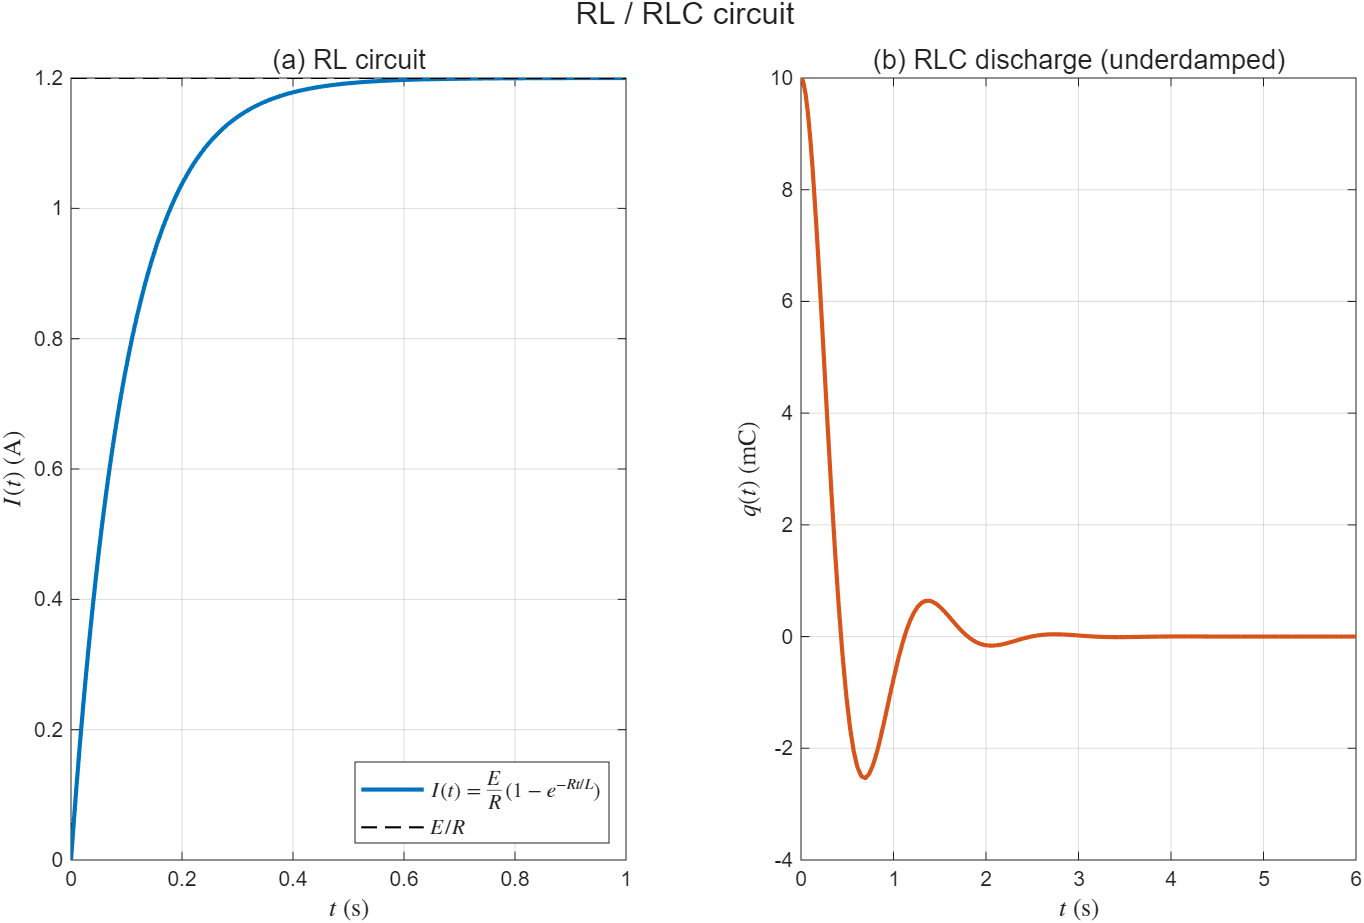
\includegraphics[width=0.92\textwidth]{Figures/RL_RLC电路.png}
    \caption{RL 串联电路电流响应与 RLC 放电（欠阻尼）曲线。MATLAB 代码见 \texttt{MATLAB代码/RL\_RLC电路.m}。}
    \label{fig:RL_RLC}
\end{figure}

\subsection{数学摆}

数学摆（单摆）满足 $\dfrac{d^2\theta}{dt^2} + \dfrac{g}{l}\sin\theta = 0$，其运动可用 MATLAB 数值求解；当摆角较小时可作小角度近似 $\sin\theta \approx \theta$，解为 $\theta(t) = \theta_0\cos\omega t$。

\begin{figure}[htbp]
    \centering
    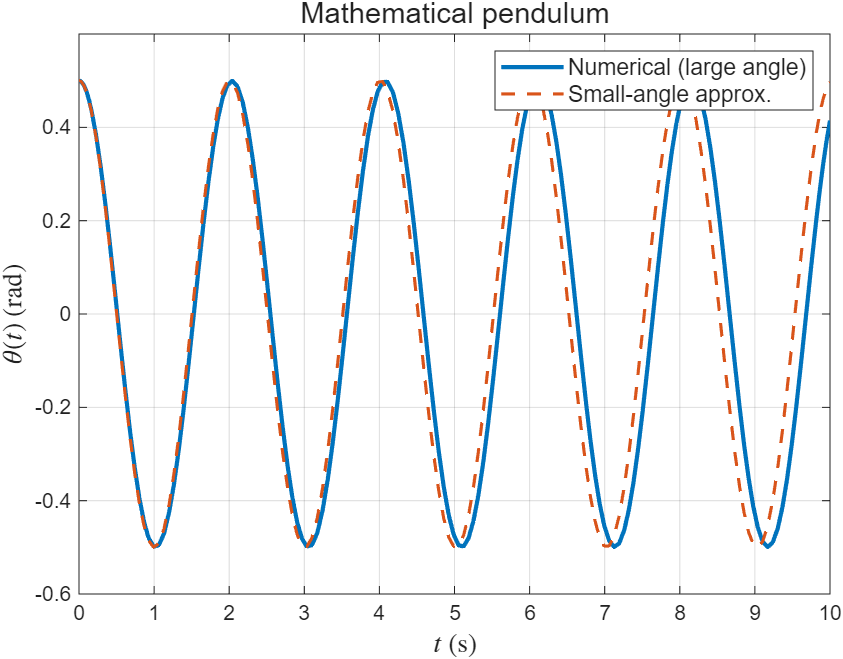
\includegraphics[width=0.75\textwidth]{Figures/数学摆.png}
    \caption{数学摆大摆角数值解与小角度近似的对比。MATLAB 代码见 \texttt{MATLAB代码/数学摆.m}。}
    \label{fig:pendulum}
\end{figure}

\subsection{人口模型（Malthus）}

假设：人口自然增长中，净相对增加率（单位时间净增长数 $/$ 人口总数）为常数 $r$。此时 $\dfrac{dN}{dt} = rN$，解为指数增长 $N(t) = N_0e^{rt}$。

\begin{figure}[htbp]
    \centering
    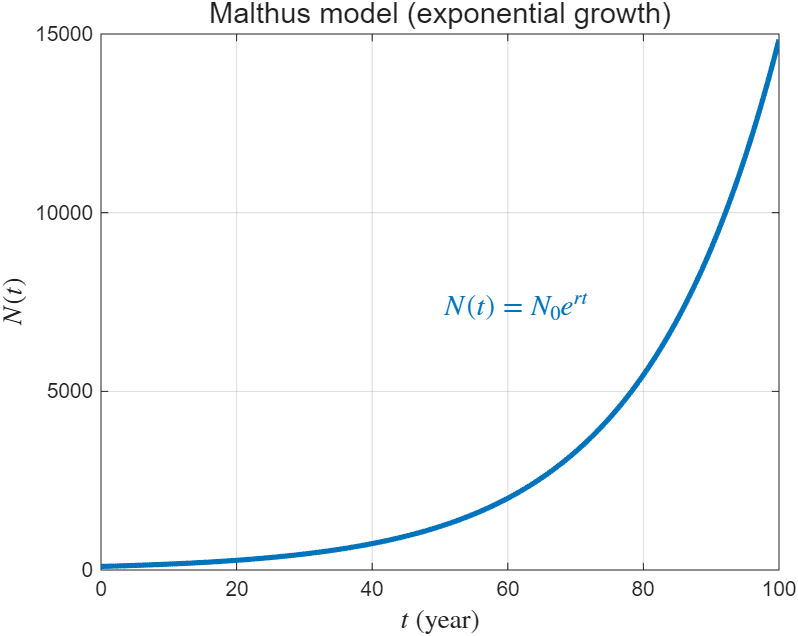
\includegraphics[width=0.65\textwidth]{Figures/Malthus人口模型.png}
    \caption{Malthus 人口模型的指数增长曲线。MATLAB 代码见 \texttt{MATLAB代码/Malthus人口模型.m}。}
    \label{fig:malthus}
\end{figure}

\subsection{人口模型的改进：logistic 模型（Verhulst）}

引入环境最大容纳量 $N_m$，假设净相对增长率为
$$r\left(1 - \frac{N(t)}{N_m}\right)$$
即 $\dfrac{dN}{dt} = rN\left(1 - \dfrac{N}{N_m}\right)$，其解为 S 形增长曲线，当 $t\to\infty$ 时 $N(t)\to N_m$。

\begin{figure}[htbp]
    \centering
    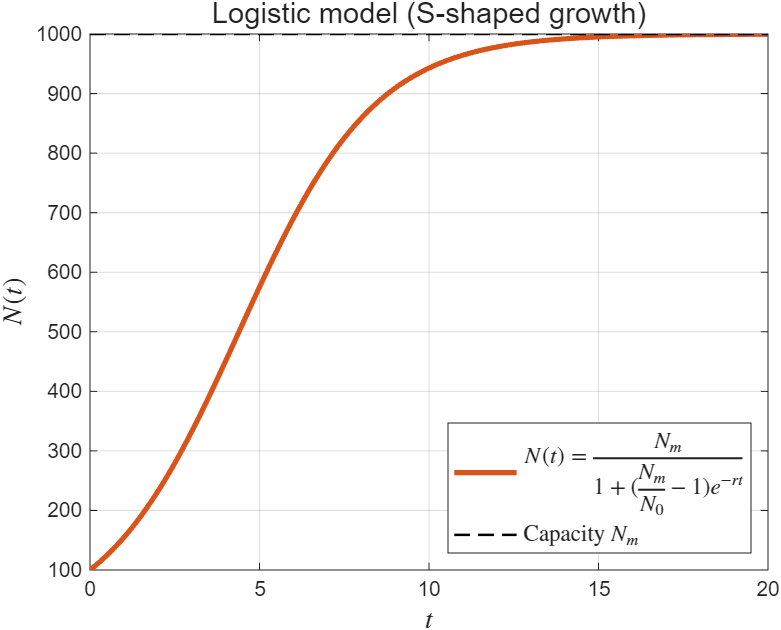
\includegraphics[width=0.65\textwidth]{Figures/Logistic模型.png}
    \caption{logistic 模型的 S 形增长曲线。MATLAB 代码见 \texttt{MATLAB代码/Logistic模型.m}。}
    \label{fig:logistic}
\end{figure}

\subsection{SI 传染病模型}

易感染者（Susceptible）与已感染者（Infective）两类，总人口 $N = S + I$ 恒定。设感染率为 $\beta$，则
$$\frac{dS}{dt} = -\beta SI, \qquad \frac{dI}{dt} = \beta SI$$

\begin{figure}[htbp]
    \centering
    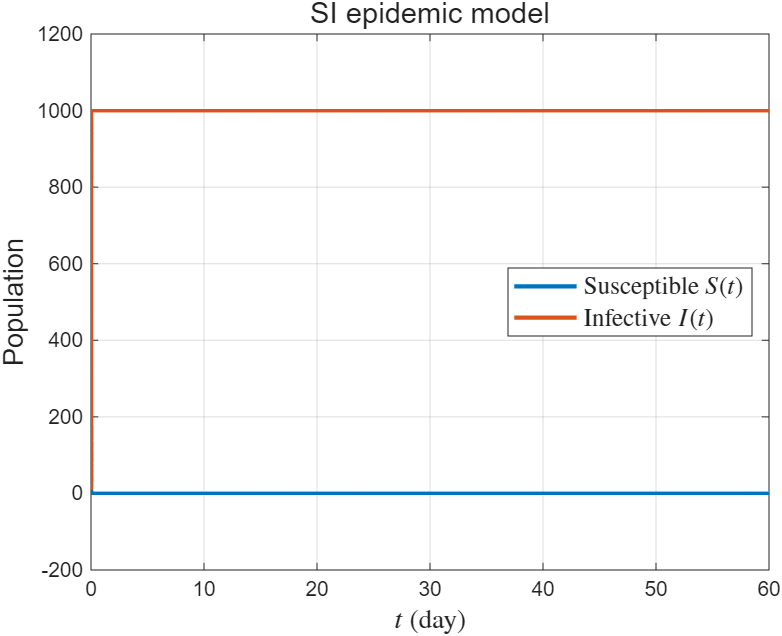
\includegraphics[width=0.65\textwidth]{Figures/SI传染病模型.png}
    \caption{SI 传染病模型中易感者与感染者人数随时间的变化。MATLAB 代码见 \texttt{MATLAB代码/SI传染病模型.m}。}
    \label{fig:SI}
\end{figure}

\subsection{Volterra 被捕食--捕食模型}

时刻 $t$ 被食鱼总数 $x(t)$，捕食鱼总数 $y(t)$；单位时间相遇次数 $bxy$；捕食鱼自然减少率与 $y$ 成正比。模型为
$$\frac{dx}{dt} = ax - bxy, \qquad \frac{dy}{dt} = -cy + dxy$$
其解呈周期振荡，相图为闭合轨线。另有两种群竞争模型。

\begin{figure}[htbp]
    \centering
    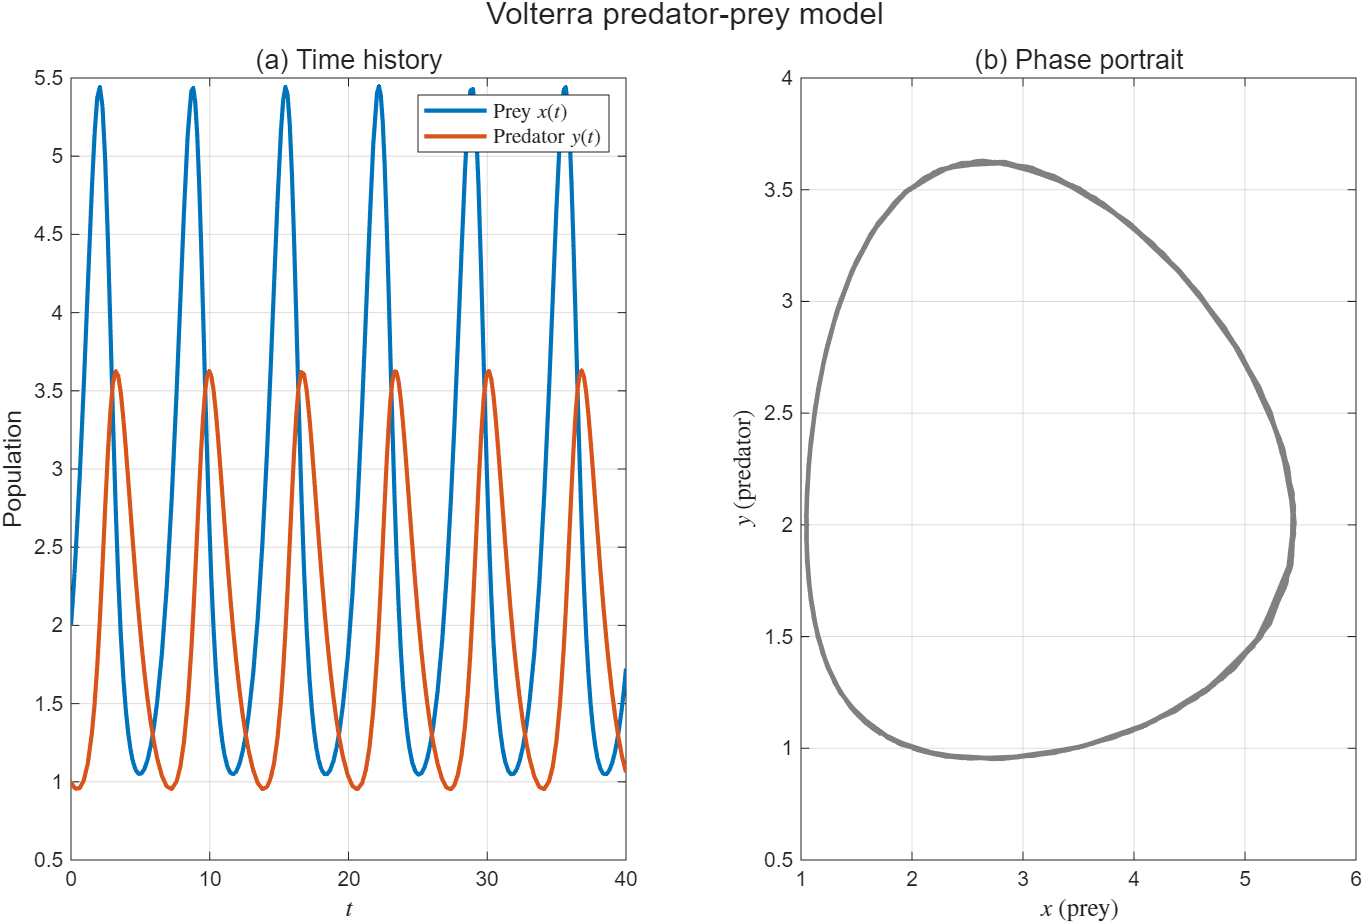
\includegraphics[width=0.92\textwidth]{Figures/Volterra捕食被捕食模型.png}
    \caption{Volterra 被捕食-捕食模型的时间历程与相图。MATLAB 代码见 \texttt{MATLAB代码/Volterra捕食被捕食模型.m}。}
    \label{fig:volterra}
\end{figure}

\subsection{Lorenz 方程（蝴蝶效应）}

Edward Lorenz（1963，MIT）给出第一个混沌现象——蝴蝶效应，为大气流体动力学模型的简化常微分方程组：
$$\frac{dx}{dt} = \sigma(y - x), \qquad \frac{dy}{dt} = x(\rho - z) - y, \qquad \frac{dz}{dt} = xy - \beta z$$

\begin{figure}[htbp]
    \centering
    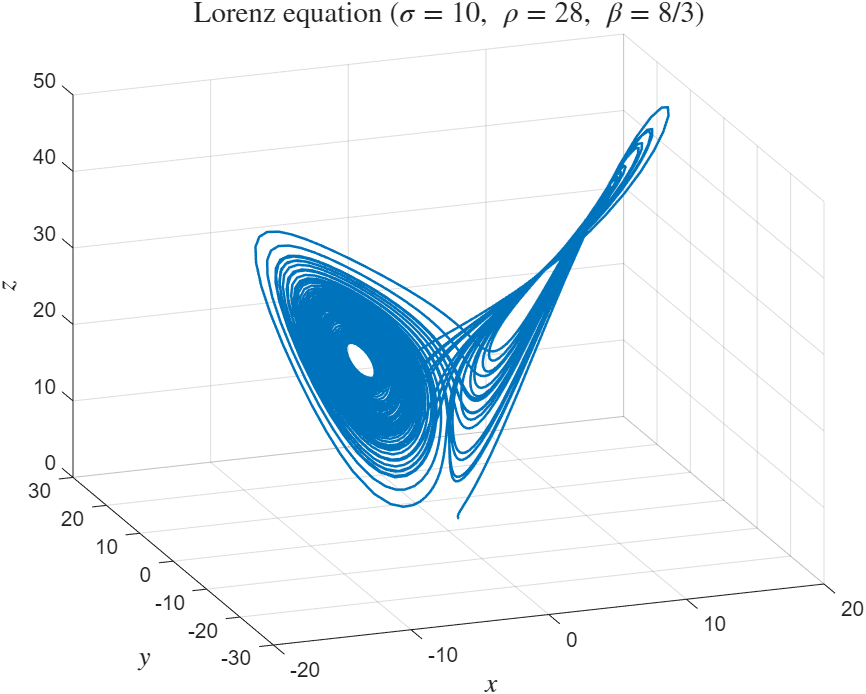
\includegraphics[width=0.7\textwidth]{Figures/Lorenz方程.png}
    \caption{Lorenz 方程的混沌吸引子（$\sigma=10,\ \rho=28,\ \beta=8/3$）。MATLAB 代码见 \texttt{MATLAB代码/Lorenz方程.m}。}
    \label{fig:lorenz}
\end{figure}

\subsection{建模总结}

微分方程反映量与量之间的关系，与时间有关，是\textbf{动态系统}。从自然规律出发，考虑主要因素，构造含自变量、未知函数及其导数的关系式 $\rightarrow$ 数学模型。研究解和解结构的性质，与实际对照，不断改进模型；可由微分方程发现或预测新规律。

\section{微分方程的基本概念}

\subsection{微分方程的定义}

联系\textbf{自变量、未知函数及未知函数的导数（或微分）}的关系式称为微分方程。

\begin{example}
下列关系式都是微分方程：
\begin{align}
\frac{dy}{dx} &= x^2 \tag{1} \\
x\,dy - y\,dx &= 0 \tag{2} \\
\frac{d^2x}{dt^2} + tx\left(\frac{dx}{dt}\right)^3 + x &= 0 \tag{3} \\
\frac{d^4x}{dt^4} + 5\frac{d^2x}{dt^2} + 3x &= \sin t \tag{4} \\
\frac{\partial z}{\partial x} + \frac{\partial z}{\partial y} &= z \tag{5} \\
\frac{\partial^2 u}{\partial x^2} + \frac{\partial^2 u}{\partial y^2} + xy - u &= 0 \tag{6}
\end{align}
\end{example}

\subsection{常微分方程与偏微分方程}

\begin{itemize}
    \item \textbf{常微分方程（ODE）}：自变量个数只有一个。例：(1)--(4)。
    \item \textbf{偏微分方程（PDE）}：自变量个数为两个或两个以上。例：(5)(6)。
    \item 注：本课程主要研究常微分方程，简称微分方程或方程。
\end{itemize}

\subsection{微分方程的阶}

微分方程中出现的\textbf{未知函数的最高阶导数（或微分）的阶数}称为微分方程的阶数。(1) 一阶；(2) 一阶；(3) 二阶；(4) 四阶。

$n$ 阶微分方程的一般形式：
$$F\left(x, y, \frac{dy}{dx}, \ldots, \frac{d^n y}{dx^n}\right) = 0$$
其中 $x$ 是自变量，$y$ 是未知函数，且一定含有 $\dfrac{d^n y}{dx^n}$。

\subsection{线性与非线性}

如果方程 $F\left(x, y, \dfrac{dy}{dx}, \ldots, \dfrac{d^n y}{dx^n}\right) = 0$ 的左端是 $y, y', \ldots, y^{(n)}$ 的一次有理式，则称为 $n$ 阶线性方程；否则为非线性方程。

$n$ 阶线性微分方程的一般形式：
$$a_n(x)\frac{d^n y}{dx^n} + a_{n-1}(x)\frac{d^{n-1} y}{dx^{n-1}} + \cdots + a_1(x)\frac{dy}{dx} + a_0(x)y = f(x)$$
其中 $a_n(x), \ldots, a_1(x), a_0(x), f(x)$ 为 $x$ 的已知函数。

线性：(1)(2)(4)；非线性：(3)（含 $\left(\frac{dx}{dt}\right)^3$ 项）。

\subsection{微分方程的解}

\begin{mydefinition}{定义}
若函数 $y = \varphi(x)$ 在区间 $I$ 上有直到 $n$ 阶的连续导数，且对 $\forall x \in I$ 有
$$F\left(x, \varphi(x), \varphi'(x), \ldots, \varphi^{(n)}(x)\right) \equiv 0$$
则称 $y = \varphi(x)$ 为方程在 $I$ 上的一个解，称为\textbf{显式解}。
\end{mydefinition}

\begin{example}
验证 $y = \sin x$ 与 $y = \cos x$ 都是 $y'' + y = 0$ 在 $(-\infty, +\infty)$ 上的解。

（$y = \sin x \Rightarrow y' = \cos x, y'' = -\sin x \Rightarrow y'' + y = -\sin x + \sin x = 0$ $\checkmark$）
\end{example}

\subsection{显式解与隐式解}

若关系式 $\Phi(x, y) = 0$ 确定的隐函数 $y = \varphi(x)$ 是方程的解，则称 $\Phi(x, y) = 0$ 为方程的\textbf{隐式解}。

\begin{example}
一阶方程 $\dfrac{dy}{dx} = - \dfrac{x}{y}$ 有显式解 $y = -\sqrt{1-x^2}$ 与 $y = \sqrt{1-x^2}$，隐式解 $x^2 + y^2 = 1$。
\end{example}

\begin{remark}
显式解与隐式解统称为微分方程的解。
\end{remark}

\subsection{通解与特解}

\begin{mydefinition}{定义}
若微分方程的解中含有任意常数，且所含\textbf{相互独立的任意常数的个数与方程的阶数相同}，则称为方程的\textbf{通解}。
\end{mydefinition}

\begin{example}
$y = c_1 \sin x + c_2 \cos x$（$c_1, c_2$ 为任意常数）是 $y'' + y = 0$ 的通解。
\end{example}

$n$ 阶微分方程通解的一般形式：
$$y = \varphi(x, c_1, c_2, \ldots, c_n)$$
其中 $c_1, \ldots, c_n$ 为相互独立的任意常数（独立性的行列式判别条件：Wronski 型行列式 $\neq 0$）。

\begin{example}
验证 $y = c_1 e^x + c_2 e^{-x} + c_3 e^{2x} + \dfrac{1}{2}$ 是 $y''' - 2y'' - y' + 2y = 6$ 的通解（代入计算可证，且 Wronski 行列式非零）。
\end{example}

\begin{itemize}
    \item \textbf{隐式通解（通积分）}：隐式解中含有任意常数且个数与阶数相同。
    \item 以后不区分显式通解与隐式通解，统称\textbf{通解}。
\end{itemize}

\textbf{特解}：在通解中给任意常数以确定的值而得到的解。

\begin{example}
通解 $y = c_1 \sin x + c_2 \cos x$ 中取 $c_1 = 0, c_2 = 1$ 得 $y = \cos x$；取 $c_1 = 1, c_2 = 0$ 得 $y = \sin x$，均为 $y'' + y = 0$ 的特解。
\end{example}

\subsection{定解条件与初值问题（Cauchy 问题）}

\begin{itemize}
    \item \textbf{定解条件}：根据实际问题附加的条件；求满足定解条件的解的问题称\textbf{定解问题}。
    \item \textbf{初始条件}：$n$ 阶微分方程的初始条件指 $n$ 个条件（当 $x = x_0$ 时）：
    $$y(x_0) = y_0, \quad y'(x_0) = y_0^{(1)}, \quad \ldots, \quad y^{(n-1)}(x_0) = y_0^{(n-1)}$$
    其中 $x_0, y_0, y_0^{(1)}, \ldots, y_0^{(n-1)}$ 为给定的 $n+1$ 个常数。
    \item 定解条件为初始条件时，相应定解问题称为\textbf{初值问题（Cauchy 问题）}。
\end{itemize}

\begin{example}
验证 $y = c_1 e^{-x} + c_2 e^{-4x}$ 是 $y'' + 5y' + 4y = 0$ 的通解，并求满足 $y(0) = 2, y'(0) = 1$ 的特解。
\end{example}

\begin{solution}
特征方程 $\lambda^2 + 5\lambda + 4 = 0$ 的根为 $\lambda = -1, -4$，故 $e^{-x}, e^{-4x}$ 是对应齐次方程的两个线性无关解，$y = c_1 e^{-x} + c_2 e^{-4x}$ 确为其通解。由初始条件得方程组
$$\begin{cases} c_1 + c_2 = 2 \\ -c_1 - 4c_2 = 1 \end{cases} \Rightarrow c_1 = 3, \; c_2 = -1$$
故所求特解为 $y = 3e^{-x} - e^{-4x}$。
\end{solution}

\subsection{积分曲线与方向场}

\begin{itemize}
    \item \textbf{积分曲线}：一阶方程 $\dfrac{dy}{dx} = f(x, y)$ 的解 $y = \varphi(x)$ 在 $xy$ 平面上表示的曲线；通解对应一族积分曲线。
    \item \textbf{方向场}：在 $f(x, y)$ 的定义域 $D$ 内每一点画一个以 $f(x, y)$ 为斜率、中心在该点的直线段，带有这种直线段的区域称为方程的方向场。
    \item \textbf{等斜线}：方向场中方向相同的点的几何轨迹。方程 $\dfrac{dy}{dx} = f(x, y)$ 的等斜线为 $f(x, y) = k$（$k$ 为参数）。
\end{itemize}

\subsection{微分方程组}

略（详见第五章）。

\subsection{驻定（自治）与非驻定（非自治）}

\begin{itemize}
    \item 驻定（自治）系统：右端不显含自变量。
    \item 非驻定（非自治）系统：右端显含自变量。
\end{itemize}

\subsection{相空间、轨线与奇点}

\begin{itemize}
    \item \textbf{相空间}：不含自变量、仅由未知函数组成的空间。
    \item \textbf{轨线}：积分曲线在相空间中的投影。
    \item \textbf{奇点（平衡点）}：平衡解（驻定解、常数解）对应的点。
\end{itemize}

\begin{example}
$\begin{cases} \dot{u} = v \\ \dot{v} = -u \end{cases}$，$u(0) = 1, v(0) = 0$ 的解为 $(u(t), v(t)) = (\cos t, -\sin t)$，轨线为相平面中的圆（$u^2 + v^2 = 1$）。
\end{example}

\subsection{垂直等倾线、水平等倾线}

略（详见第六章）。

\section*{作业}

\begin{itemize}
    \item p12：1（1、3、6）
    \item p13：3（1、5、8），4，6，7
\end{itemize}
